%
% Main document
% ===========================================================================
\documentclass[
    paper=a4,               % paper format
    fontsize=10pt,          % fontsize
    %twoside,               % double-sided
    open=right,             % begin new chapter on right side
    titlepage=false,        % use no standard title page
    parskip=half,           % set paragraph skip to half of a line
]{scrreprt}                 % KOMA-script report
%---------------------------------------------------------------------------
\raggedbottom{}
%\KOMAoptions{cleardoublepage=plain}                                    % Add header and footer on blank pages


% Load Standard Packages:
%---------------------------------------------------------------------------
\usepackage{scrpage2}
\usepackage{pgfgantt}
\usepackage[standard-baselineskips]{cmbright}

\usepackage{scrhack}
\usepackage[ngerman]{babel}                                             % german hyphenation
\usepackage[utf8]{inputenc}                                             % UTF-8 character encoding
\usepackage[T1]{fontenc}                                                % hyphenation of words with ä,ö and ü
\usepackage{textcomp}                                                   % additional symbols
% \usepackage{ae}                                                         % better resolution of Type1-Fonts 
% \usepackage{fancyhdr}                                                   % simple manipulation of header and footer 
\usepackage{etoolbox}                                                   % color manipulation of header and footer
\usepackage{graphicx}                                                   % integration of images
\usepackage{float}                                                      % floating objects
\usepackage{caption}                                                    % for captions of figures and tables
\usepackage{booktabs}                                                   % package for nicer tables
\usepackage{tocvsec2}                                                   % provides means of controlling the sectional numbering
\usepackage[round,sort,comma,authoryear]{natbib}                          % provides various citation styles
\usepackage{wrapfig}                                                    % provides floating of text around images
\usepackage{nameref}                                                    % provides printing names of references
\usepackage{paralist}
%---------------------------------------------------------------------------

% Definition of Colors
%---------------------------------------------------------------------------
\RequirePackage{color}                                                  % Color (not xcolor!)
\definecolor{linkblue}{rgb}{0,0,0.8}                                    % Standard
\definecolor{darkblue}{rgb}{0,0.08,0.45}                                % Dark blue
\definecolor{bfhgrey}{rgb}{0.41,0.49,0.57}                              % BFH grey
%\definecolor{linkcolor}{rgb}{0,0,0.8}                                  % Blue for the web- and cd-version!
\definecolor{linkcolor}{rgb}{0,0,0}                                     % Black for the print-version!
\definecolor{codecommentcolor}{rgb}{0, 0.6, 0}                          % Color for code comments
\definecolor{black}{rgb}{0, 0, 0}
\definecolor{maroon}{rgb}{0.5,0,0}
\definecolor{darkgreen}{rgb}{0,0.5,0}
\definecolor{darkblue}{rgb}{0.0,0.0,0.6}
%---------------------------------------------------------------------------

% Load listings package
% which provides source code formatting
%---------------------------------------------------------------------------
\usepackage{listings}                                                   % provides source code formatting
% Define XML colors
\lstdefinelanguage{XML}
{basicstyle=\ttfamily\footnotesize,
  morestring=[b]'',
  moredelim=[s][\bfseries\color{maroon}]{<}{\ },
  moredelim=[s][\bfseries\color{maroon}]{</}{>},
  moredelim=[l][\bfseries\color{maroon}]{/>},
  moredelim=[l][\bfseries\color{maroon}]{>},
  morecomment=[s]{<?}{?>},
  morecomment=[s]{<!--}{-->},
  commentstyle=\color{codecommentcolor},
  stringstyle=\color{darkblue},
  identifierstyle=\color{red}
}
%---------------------------------------------------------------------------

% Comment package
%---------------------------------------------------------------------------
\usepackage{comment}
%---------------------------------------------------------------------------

% Load Math Packages
%---------------------------------------------------------------------------
\usepackage{amsmath}                                                    % various features to facilitate writing math formulas
\usepackage{amsthm}                                                     % enhanced version of latex's newtheorem
\usepackage{amsfonts}                                                   % set of miscellaneous TeX fonts that augment the standard CM
\usepackage{amssymb}                                                    % mathematical special characters
\usepackage{exscale}                                                    % mathematical size corresponds to textsize
%---------------------------------------------------------------------------

% Package to facilitate placement of boxes at absolute positions
%---------------------------------------------------------------------------
\usepackage[absolute]{textpos}
\setlength{\TPHorizModule}{1mm}
\setlength{\TPVertModule}{1mm}
%---------------------------------------------------------------------------

% Package for annotations
% See http://ctan.mirrorcatalogs.com/macros/latex/contrib/ed/ed.pdf
%---------------------------------------------------------------------------
\usepackage[hide]{ed}
%---------------------------------------------------------------------------

% Hyperref Package (Create links in a pdf)
%---------------------------------------------------------------------------
\usepackage[
    pdftex,ngerman,bookmarks,plainpages=false,pdfpagelabels,
    backref = {false},                                                  % No index backreference
    colorlinks = {true},                                                % Color links in a PDF
    hypertexnames = {true},                                             % no failures "same page(i)"
    bookmarksopen = {true},                                             % opens the bar on the left side
    bookmarksopenlevel = {0},                                           % depth of opened bookmarks
    pdftitle = {Kommunikationsanalyse},                          % PDF-property
    pdfauthor = {ostes2},                                                 % PDF-property
    pdfsubject = {Projektarbeit},                                      % PDF-property
    linkcolor = {linkcolor},                                            % Color of Links
    citecolor = {linkcolor},                                            % Color of Cite-Links
    urlcolor = {linkcolor},                                             % Color of URLs
]{hyperref}
%---------------------------------------------------------------------------

% Cross-reference package
%---------------------------------------------------------------------------
\usepackage{xr}                                                         % provides references to other, external documents
%---------------------------------------------------------------------------
% Set up page dimension
%---------------------------------------------------------------------------
\usepackage{geometry}
\geometry{a4paper,
    left=28mm,
    right=15mm,
    top=30mm,
    headheight=20mm,
    headsep=10mm,
    textheight=242mm,
    footskip=15mm
}
%---------------------------------------------------------------------------

% Makeindex Package
%---------------------------------------------------------------------------
\usepackage{makeidx}                                % To produce index
\makeindex                                      % Index-Initialisation
%---------------------------------------------------------------------------

% Glossary Package
%---------------------------------------------------------------------------
% the glossaries package uses makeindex
% if you use TeXnicCenter do the following steps:
%  - Goto "Ausgabeprofile definieren" (ctrl + F7)
%  - Select the profile "LaTeX => PDF"
%  - Add in register "Nachbearbeitung" a new "Postprozessoren" point named Glossar
%  - Select makeindex.exe in the field "Anwendung" ( ..\MiKTeX x.x\miktex\bin\makeindex.exe )
%  - Add this [ -s "%tm.ist" -t "%tm.glg" -o "%tm.gls" "%tm.glo" ] in the field "Argumente"
%
% for futher informations go to http://ewus.de/tipp-1029.html
%---------------------------------------------------------------------------
\usepackage[nonumberlist]{glossaries}
\makeglossaries{}
\newglossaryentry{aktiver Konturen}
{
    name=Aktive Konturen,
    description={Foos the bar}
}

\newglossaryentry{Segmentationsmethoden}
{
    name=Segmentation,
    description={``Segmentieren beduetet, jedes Pixel einer bestimmten Region zuzuweisen.''~\cite[S. 133]{hudritsch:script:cp}}
}

%---------------------------------------------------------------------------

% Intro:
%---------------------------------------------------------------------------
%\begin{document}                                % Start Document
\settocdepth{section}                                                       % Set depth of toc
\pagenumbering{roman}                                                       
%---------------------------------------------------------------------------

\providecommand{\doctitle}{Kommunikationsanalyse}
                  % Titel der Arbeit aus Datei titel.tex lesen
% Current version number
\providecommand{\versionnumber}{0.1}

% Date of the current version
\providecommand{\versiondate}{{\today}}
                % Versionsnummer und -datum aus Datei version.tex lesen

% Set up header and footer
%---------------------------------------------------------------------------

\deftripstyle{newlayout}
  [0pt] % no header line
  [0pt] % no footer line
  {}
  {}
  {}
  {\color{bfhgrey} \footnotesize \doctitle, Version \versionnumber, \versiondate}
  {}
  {\color{bfhgrey} \thepage}

\pagestyle{newlayout}
% use "pagestyle" also on chapter starting pages 
\renewcommand{\chapterpagestyle}{newlayout}
\renewcommand{\chaptermark}[1]{\markboth{\thechapter.  #1}{}}
\renewcommand*{\headfont}{\normalfont}
\renewcommand*{\footfont}{\normalfont}
%---------------------------------------------------------------------------

% Randnotizen
\newcommand\mpar[1]{\marginpar{\flushleft\sffamily\small #1}}
\setlength{\marginparwidth}{1.5cm}

\color{black}
\begin{document}

\lstset{language=XML,
  caption={},
  frame=L,
  basicstyle=\small\normalfont\sffamily,  % the size of the fonts that are used for the code
  stepnumber=1,                           % the step between two line-numbers.
                                          % If it is 1 each line will be numbered
  numbersep=10pt,                         % how far the line-numbers are from the code
  tabsize=2,                              % tab size in blank spaces
  extendedchars=true,                     %
  breaklines=true,                        % sets automatic line breaking
  captionpos=b,                           % sets the caption-position to bottom
  mathescape=true,
  showspaces=false,                       % Leerzeichen anzeigen ?
  showtabs=false,                         % Tabs anzeigen ?
  xleftmargin=17pt,
  framexleftmargin=17pt,
  framexrightmargin=17pt,
  framexbottommargin=5pt,
  framextopmargin=5pt,
  showstringspaces=false                  % Leerzeichen in Strings anzeigen ?
  belowcaptionskip=5em,
  belowskip=3em,
  aboveskip=3em
 }

% Make sure Umlauts are getting displayed correctly.
\lstset{literate=%
    {Ö}{\textcolor{red}{\"O}}1
    {Ä}{{\"A}}1
    {Ü}{{\"U}}1
    {ß}{{\ss}}1
    {ü}{{\"u}}1
    {ä}{{\textcolor{red}{\"a}}}1
    {ö}{{\textcolor{red}{\"o}}}1
    {~}{{\textasciitilde}}1
    {?}{{\textcolor{red}{?}}}1
}

% Title Page and Abstract
%---------------------------------------------------------------------------
\begin{titlepage}

\setlength{\unitlength}{1mm}
\begin{textblock}{20}[0,0](28,12) % chktex-file 36
    
\includegraphics[scale=1.0]{images/BFH_Logo_B.png}
\end{textblock}

\begin{textblock}{154}(28,48)
    \begin{picture}(150,2)
        \put(0,0){\color{bfhgrey}\rule{150mm}{2mm}}
    \end{picture}
\end{textblock}

\begin{textblock}{154}[0,0](26.7,50.5)
    \centering
    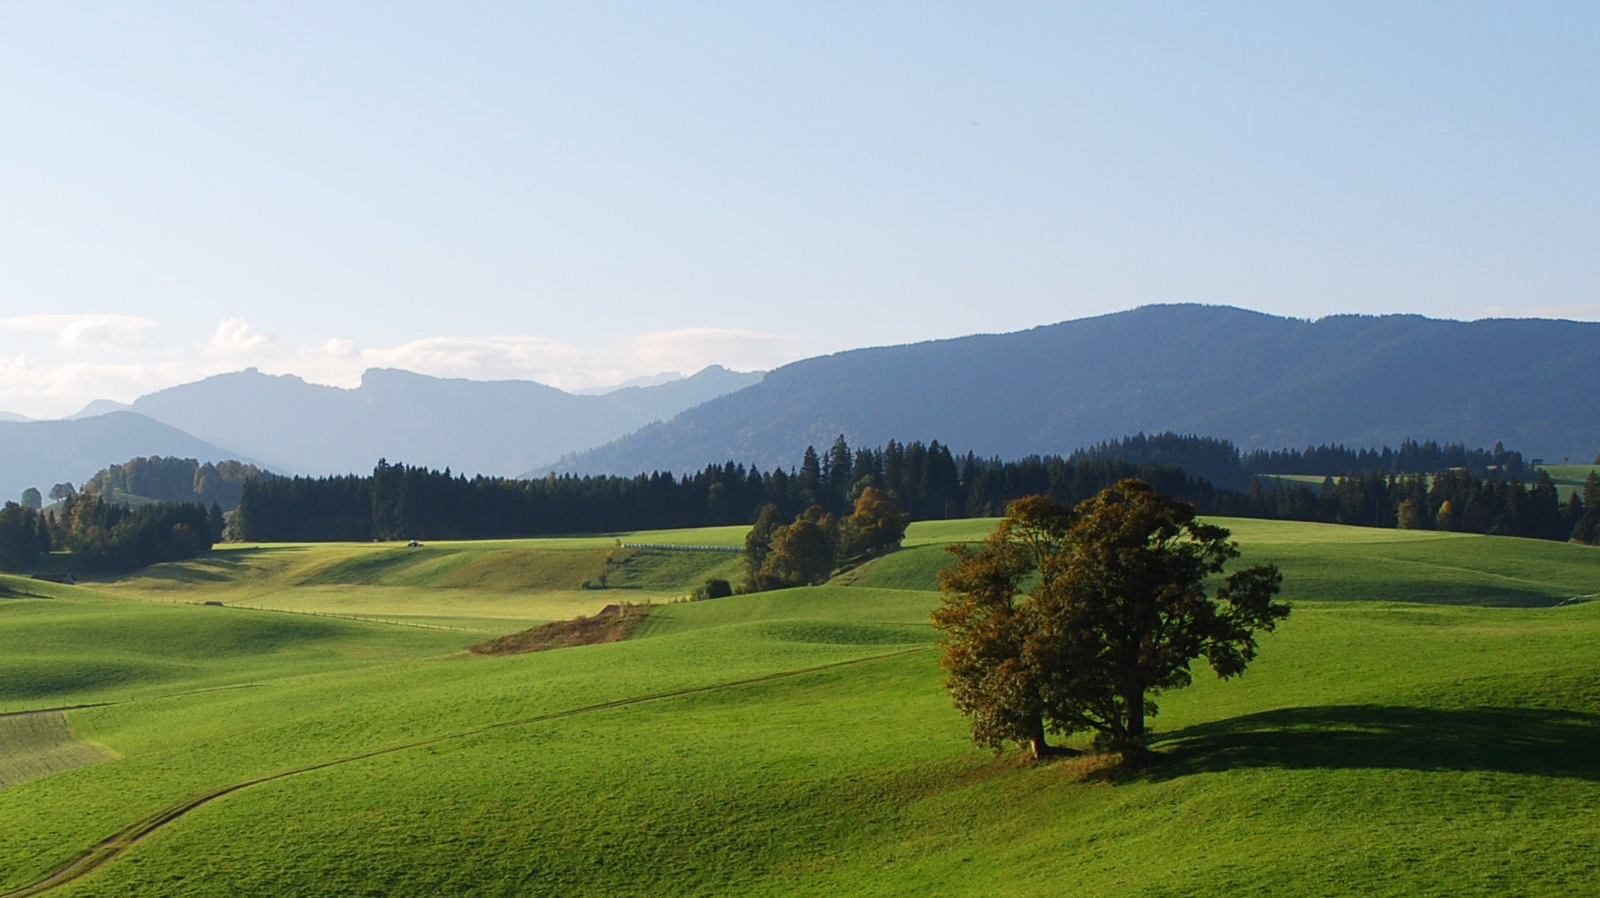
\includegraphics[scale=0.264]{images/title.jpg}\protect\footnotemark{}
\end{textblock}
\footnotetext{Quelle: \url{http://www.freeimages.com/photo/1241246}}

\begin{textblock}{154} (28,135)
    \begin{picture}(150,2)
        \put(0,0){\color{bfhgrey}\rule{150mm}{2mm}}
    \end{picture}
\end{textblock}
\color{black}

\begin{flushleft}

\vspace*{120mm}

\fontsize{26pt}{28pt}\selectfont
Komunikationsanalyse
\vspace{3mm}

\fontsize{20pt}{22pt}\selectfont
Projektarbeit
\vspace{3mm}

\fontsize{10pt}{12pt}\selectfont
\textbf{BZG3101: Kommunikation 1} \\
\vspace{3mm}

\begin{textblock}{150} (28,215)
\fontsize{10pt}{17pt}\selectfont
\begin{tabbing}
xxxxxxxxxxxxxxx\=xxxxxxxxxxxxxxxxxxxxxxxxxxxxxxxxxxxxxxxxxxxxxxx \kill
Autor:        \> Sven Osterwalder\\
Datum:        \> \versiondate\\
Betreuer:     \> Patrick Studer\\
\end{tabbing}

\end{textblock}
\end{flushleft}

\begin{textblock}{150} (28,280)
\noindent 
\color{bfhgrey}\fontsize{9pt}{10pt}\selectfont
Berner Fachhochschule | Haute école spécialisée bernoise | Bern University of Applied Sciences
\color{black}\selectfont
\end{textblock}


\end{titlepage}

\cleardoublepage{}
\phantomsection{}
\chapter*{}
\label{chap:versionen}

\begin{textblock}{180} (15,150)
\color{black}
\begin{huge}
Versionen
\end{huge}
\vspace{10mm}

\fontsize{10pt}{18pt}\selectfont
\begin{tabbing}
xxxxxxxxxxx\=xxxxxxxxxxxxxxx\=xxxxxxxxxxxxxx\=xxxxxxxxxxxxxxxxxxxxxxxxxxxxxxxxxxxxxxxxxxxxxxx \kill
\textit{Version}	\> \textit{Kalenderwoche}	\> \textit{Status}		\> \textit{Bemerkungen}\\
0.1	\> 9	\> Entwurf		\> Initiale Erstellung des Dokuments\\
0.2	\> 10	\> Entwurf		\> Erstellung Konzept\\
0.3	\> 11	\> Entwurf		\> Verfassen der Einleitung und Grundlagen\\
\end{tabbing}

\end{textblock}

\phantomsection{}
\cleardoubleemptypage{}
\setcounter{page}{1}
\cleardoublepage{}
\phantomsection{}
%\addcontentsline{toc}{chapter}{Versionen}
\cleardoubleemptypage{}
%---------------------------------------------------------------------------

% Summary
%---------------------------------------------------------------------------
\chapter{Zusammenfassung}
\label{chap:summary}

% Die Zusammenfassung wird am zweithäufigsten gelesen. Danach entscheiden viele Leute, ob sie den Bericht weiterlesen oder nicht. In der Zusammenfassung werden Fragestellung und Hypothesen, Methoden, Ergebnisse und Schlussfolgerungen möglichst kurz dargestellt (jeweils etwa zwei bis drei Sätze).

[TODO:\@ Management-Summary hier einfügen wenn fertig]


% Table of contents
%---------------------------------------------------------------------------
\tableofcontents
% \cleardoublepage{}
%---------------------------------------------------------------------------

% Main part
%---------------------------------------------------------------------------
\pagenumbering{arabic}
\chapter{Einleitung}
\label{chap:intro}

\begingroup
    \leftskip=4em
    \rightskip\leftskip{}
    \textit{``Man kann nicht nicht kommunizieren, denn jede Kommunikation (nicht nur mit Worten) ist Verhalten und genauso wie man sich nicht nicht verhalten kann, kann man nicht nicht kommunizieren.''}~\cite{watzlawick2011menschliche}
    \par
\endgroup

Diese Projektarbeit ist Teil eines Projektes im Rahmen des Moduls \textit{BZG3101: Kommunikation 1 Deutsch} der Berner Fachhochschule für angewandte Wissenschaft.

Das Ziel dieser Projektarbeit ist die Erstellung und Analyse eines kommunikativen Profils sowie die Analyse der direkten und indirekten unternehmensinternen Kommunikation von Sven Osterwalder.

Im ersten Teil der Arbeit erfolgt eine Erstellung und Analyse des persönlichen kommunikativen Profils. Im zweiten Teil der Arbeit wird die unternehmensinterne Kommunikation beobachtet und analysiert. Im letzten Teil der Arbeit erfolgt eine Diskussion der gewonnenen Erkenntnisse.

%  Die Einleitung führt die Leserinnen und Leser in die Thematik der Arbeit ein. Sie setzt den Rahmen für die Arbeit, skizziert den aktuellen Wissensstand und geht auf die konkreten Fragestellungen und Ziele der vorliegenden Arbeit ein. Aus der Einleitung muss klar hervorgehen, weshalb die Arbeit gemacht wurde und welche Bedeutung ihr zukommt.
%  
%  \begin{itemize}
%      \item Ziel, worum geht es?
%      \item Eine gute Einleitung motiviert, den ganzen Bericht zu lesen.
%      \item Eine gute Einleitung enthält alle später angesprochenen Themen, aber nur diese!
%      \item Was will ich wissen?
%      \item Was habe ich für Daten? (Wie gesammelt, woher, Weiterarbeit?)
%      \item Welche Modelle brauche ich? (Matlab Toolbox)
%      \item Was erwarte ich von den Resultaten?
%  \end{itemize}

\chapter{Kommunikatives Profil}
\label{chap:analysis}

\section{Kilmann-Test}
\begin{table}[h]
    \begin{tabular}{ll}
        Kampf                  & 0          \\
        \textbf{Integration}   & \textbf{9} \\
        Kompromiss             & 5          \\
        Flucht                 & 7          \\
        \textbf{Unterdrückung} & \textbf{9}
    \end{tabular}
\end{table}

\begin{figure}[H]
    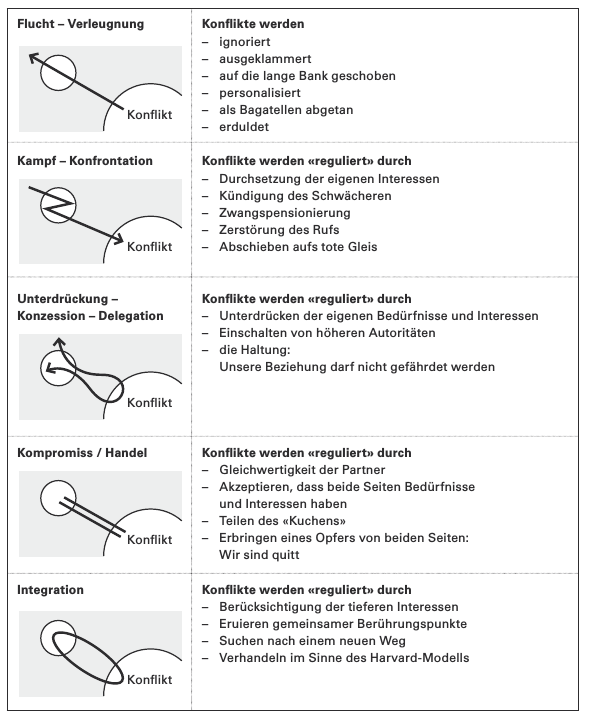
\includegraphics[scale=0.4]{images/konfliktbearbeitung_schwarz.png}
\end{figure}

\chapter{Unternehmensinterne Kommunikation}
\label{chap:observations}



\chapter{Diskussion}
\label{chap:results}

% Dieses Kapitel enthält die gewonnenen Daten und ist deshalb in wissenschaftlicher Hinsicht besonders wichtig. Es dürfen nur Ergebnisse, die für die Fragestellung relevant sind, aufgeführt werden. Dazu können aber auch Negativergebnisse gehören. Die Fragen der Einleitung müssen mit den vorgestellten Ergebnissen zu beantworten sein.
% 
% Die Ergebnisse sollten mit Hilfe von Abbildungen und Tabellen möglichst übersichtlich dargestellt werden. Der Text sollte möglichst kurz gehalten werden und nicht die Informationen der Abbildungen und Tabellen wiederholen. Emotionen wie z.B. Erstaunen oder Entsetzen sollten vermieden werden. In den statistischen Auswertungen müssen neben Mittelwerten auch Streuungsmasse und Stichprobengrössen angegeben werden.
% 
% Es muss immer klar sein, ob es sich um eigene oder fremde Ergebnisse (z.B. aus Literaturrecherchen) handelt. Bei fremden Ergebnissen muss im Text auf die Herkunft verwiesen werden (siehe 2.8). Wörtliche Zitate sollten vermieden werden.

%  \begin{compactenum}[a)] % chktex 9 chktex 10 chktex 17
%      \item Auszug aus einer zoologischen Untersuchung zur Diversität von Arthropoden in voralpinen Flachmooren:
%          „In den untersuchten Gebieten konnten 63 Tagfalterarten aus 6 Familien nachgewiesen werden (Anhang IV). 16 Arten (25\%) gelten als typische Moorindikatoren und 23 Arten (37\%) erscheinen auf der Roten Liste der gefährdeten Tagfalter der Schweiz (Duelli 1994). Die Individuenzahl der Arthropoden nahm mit zunehmender Höhe ab (p < 0.05). Während in der tiefen Höhenstufe durchschnittlich 249 Tiere pro Gebiet gefangen wurden, waren es in der mittleren Höhenstufe 236 und in der höchsten nur noch 191 Individuen.“
%      \item Auszug aus einer sozialwissenschaftlichen Untersuchung über Engagement und Mobilität:
%          „Die Gesamtmobilität der Befragten liegt bei 12'600 km (Bezugsjahr 1994). Sie hat im erfragten Zeitraum um 12\% zugenommen (von 11'300 km auf 12'600 km). Der grösste Teil dieses Anstiegs geht auf die Ferienmobilität zurück, die im Schnitt von 6'400 km auf 7'300 km zugenommen hat. Die genannten Mobilitätswerte liegen deutlich unter dem Schweizer Durchschnitt.“
%  \end{compactenum} % chktex 17

[TODO:\@ Diskussion]

%---------------------------------------------------------------------------

% Glossary
%---------------------------------------------------------------------------
\cleardoublepage{}
\phantomsection{}
\addcontentsline{toc}{chapter}{Glossar}
\renewcommand{\glossaryname}{Glossar}
\printglossary{}
%---------------------------------------------------------------------------

% Bibliography
%---------------------------------------------------------------------------
\phantomsection{}
\addcontentsline{toc}{chapter}{Literaturverzeichnis}
\bibliographystyle{unsrtnat}
\bibliography{db/bibliography}{}
%---------------------------------------------------------------------------

% Listings
%---------------------------------------------------------------------------

% \phantomsection{}
% \addcontentsline{toc}{chapter}{Abbildungsverzeichnis}
% \listoffigures

%\phantomsection{}
%\addcontentsline{toc}{chapter}{Tabellenverzeichnis}
%\listoftables
%---------------------------------------------------------------------------

% Index
%---------------------------------------------------------------------------

%\phantomsection{}
%\addcontentsline{toc}{chapter}{Stichwortverzeichnis}
%\renewcommand{\indexname}{Stichwortverzeichnis}
%\printindex
%---------------------------------------------------------------------------

% Attachment:
%---------------------------------------------------------------------------
\appendix
\settocdepth{section}
%\include{anhang/beispielanhang}
%---------------------------------------------------------------------------

%---------------------------------------------------------------------------
\end{document} % chktex 17
